\newpage
\section{Diagrammi di sequenza}
\subsection{Introduzione}
Un diagramma di sequenza è un diagramma previsto dallo standard UML, utilizzato per descrivere un particolare scenario.
Uno scenario è una determinata sequenza di azioni in cui tutte le scelte sono state già effettuate. In pratica, nel diagramma non compaiono nè scelte, né flussi alternativi.\\
Di seguito, verranno presi in considerazione i diagrammi di sequenza per i principali scenari che il team ha individuato nell'utilizzo dell'applicazione \progetto:
\begin{itemize}
	\item Ricerca di una API;
	\item Acquisto di una API;
	\item Registrazione di una API;
	\item Ricarica del saldo del conto virtuale.
\end{itemize}

\subsection{Ricerca API}

\begin{figure}[H]
	\centering
	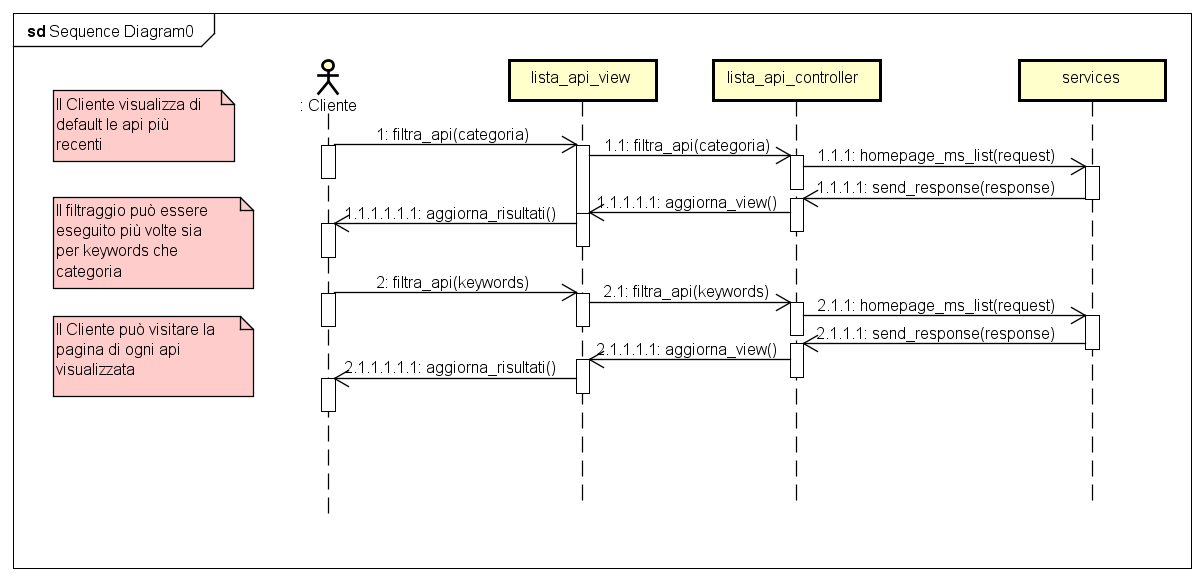
\includegraphics
	[width=0.9\linewidth]
	{UML/DiagrammiSequenza/ricerca_api.png}
	\caption{Diagramma di sequenza per la ricerca di una API}
\end{figure}

\begin{itemize}
	\item \textbf{Pre-condizioni}: l'utente si trova nella homepage dell'applicazione;
	\item \textbf{Post-condizioni}: l'utente ha visualizzato le API secondo la categoria e le keywords inserite;
	\item \textbf{Descrizione}: di default, la homepage di API Market mostra le API registrate più recentemente. L'utente può immettere delle keywords nell'apposito riquadro per alterare i risultati, e scegliere di restringere la ricerca ad una singola categoria. I risultati visualizzati cambiano dinamicamente non appena l'applicazione web riceve risposta dai servizi che la collegano ai database.
\end{itemize}

\subsection{Acquisto API}

\begin{figure}[H]
	\centering
	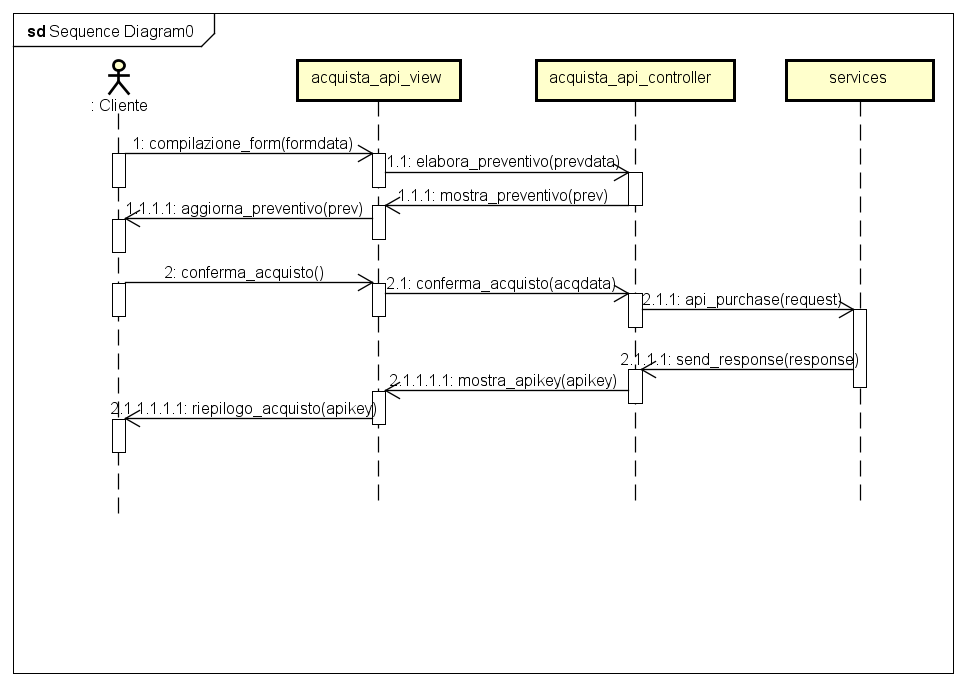
\includegraphics
	[width=0.9\linewidth]
	{UML/DiagrammiSequenza/acquisto_api.png}
	\caption{Diagramma di sequenza per l'acquisto di una API}
\end{figure}

\begin{itemize}
	\item \textbf{Pre-condizioni}: il cliente si trova nella schermata di acquisto di una specifica API;
	\item \textbf{Post-condizioni}: il cliente ha ricevuto l'API Key per l'API acquistata, secondo le modalità da lui scelte, e gli sono stati sottratti i corrispondenti crediti;
	\item \textbf{Descrizione}: il cliente compila il form per l'acquisto dell'API desiderata, visualizzando il preventivo di crediti spesi in base ai parametri scelti. Confermando l'acquisto (che può essere anche un rinnovo), i services di API Market provvedono a generare una apikey ed a scalare i crediti dall'account utente. L'utente potrà visualizzare l'API Key ed un messaggio di ringraziamento.
\end{itemize}

\subsection{Registrazione API}

\begin{figure}[H]
	\centering
	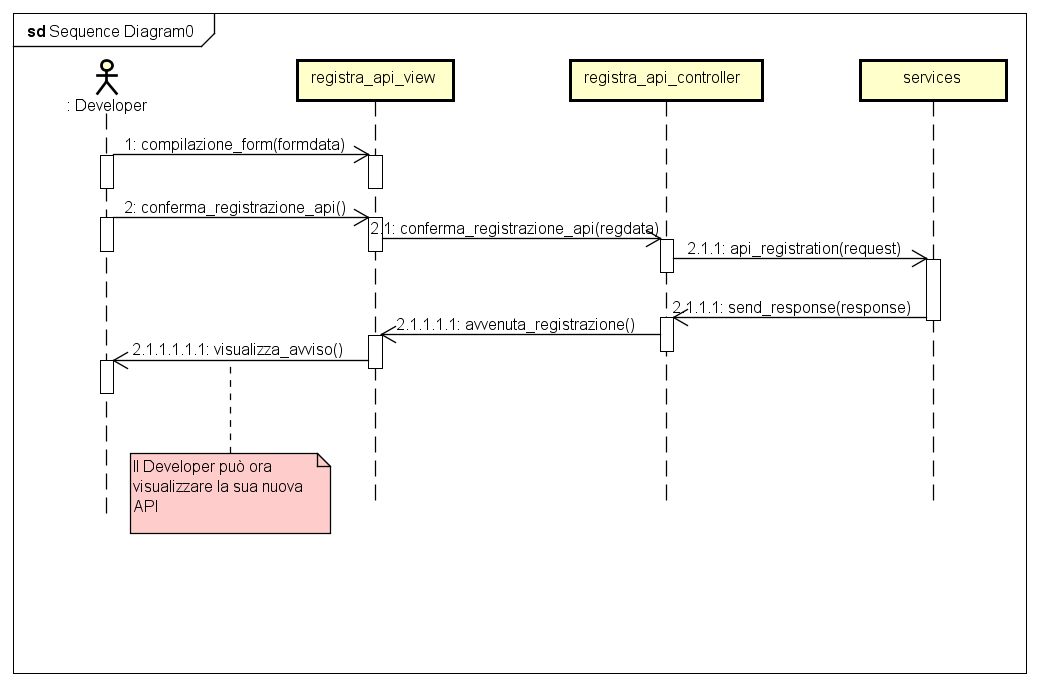
\includegraphics
	[width=0.9\linewidth]
	{UML/DiagrammiSequenza/registrazione_api.png}
	\caption{Diagramma di sequenza per la registrazione di una API}
\end{figure}

\begin{itemize}
	\item \textbf{Pre-condizioni}: lo sviluppatore si trova nella schermata di registrazione di una nuova API;
	\item \textbf{Post-condizioni}: lo sviluppatore ha registrato la sua nuova API ed essa è ora disponibile in API Market;
	\item \textbf{Descrizione}: Lo sviluppatore compila il form per la registrazione di una nuova API, provvedendo anche a caricare sul server di API Market i file del logo e della documentazione PDF. Confermando la registrazione, i services di API Market provvedono ad inserire nel database la nuova API e renderla accessibile attraverso il Gateway. A registrazione avvenuta, lo sviluppatore riceve un messaggio di successo.
\end{itemize}

\subsection{Ricarica saldo conto virtuale}

\begin{figure}[H]
	\centering
	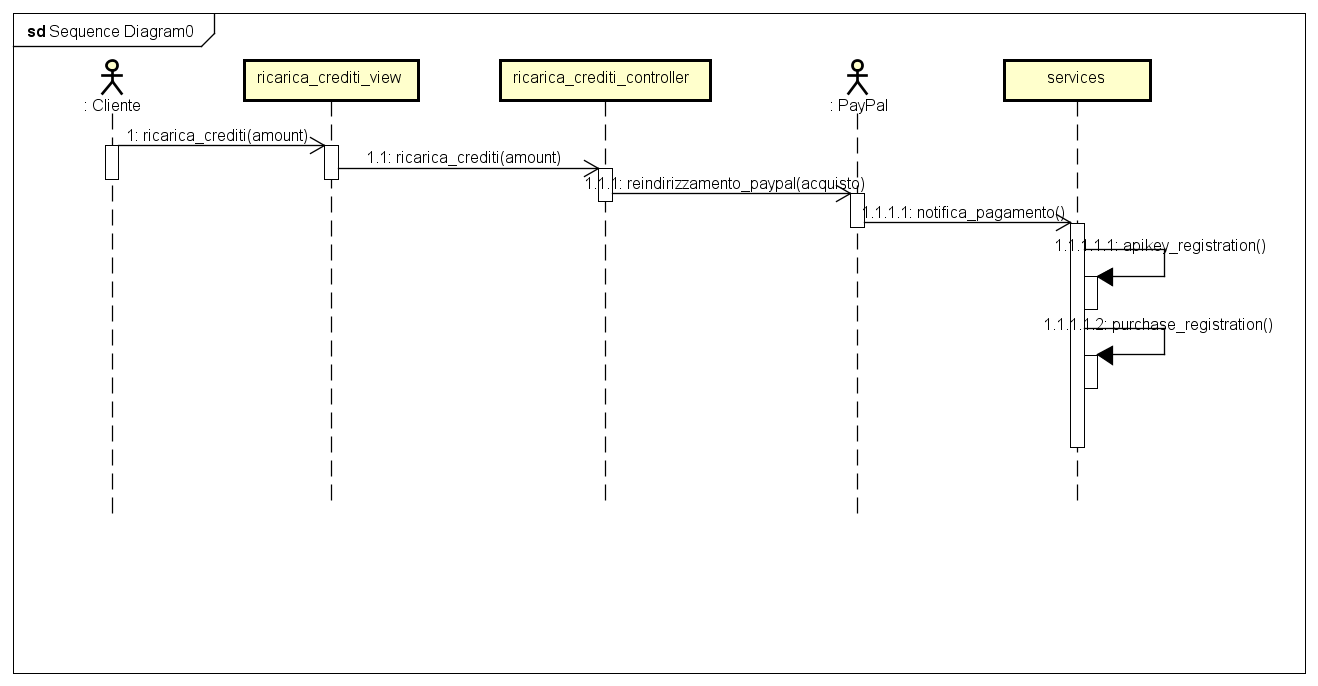
\includegraphics
	[width=0.9\linewidth]
	{UML/DiagrammiSequenza/ricarica_crediti.png}
	\caption{Diagramma di sequenza per la ricarica del saldo del conto virtuale}
\end{figure}

\begin{itemize}
	\item \textbf{Pre-condizioni}: il cliente si trova nella schermata di ricarica del proprio conto virtuale;
	\item \textbf{Post-condizioni}: il cliente ha effettuato la ricarica dei propri crediti;
	\item \textbf{Descrizione}: il cliente stabilisce l'ammontare dei crediti da ricaricare nel proprio conto virtuale. A decisione avvenuta, verrà reindirizzato alla procedura di acquisto di PayPal, che lo guiderà nell'acquisto. Portata a termine la transazione, PayPal avvertirà i services di API Market che si occuperanno di incrementare i crediti del conto virtuale del cliente.
\end{itemize}